\documentclass[12pt]{article}
\usepackage[usenames,dvipsnames]{color}
\usepackage{listings}
\usepackage{graphicx}
\usepackage{fancyhdr}
\usepackage{framed}
\usepackage[T1]{fontenc}
\usepackage[toc,page]{appendix}
\usepackage[utf8]{inputenc}
\usepackage[brazil]{babel}
\usepackage{fancyvrb}
\usepackage[hmargin=2cm,vmargin=2cm]{geometry}
\usepackage{lastpage}
\usepackage{makeidx}
\pagestyle{fancy}

% cabecalho e rodapé
\setlength{\headheight}{120pt}
\setlength{\textheight}{550pt}
\renewcommand{\headrulewidth}{0pt}
\lhead{
\includegraphics[scale=0.03]{brasao.png}}
\rhead{
\includegraphics[scale=0.4]{logo-pnud.png}}
\cfoot{\textbf{\ProjectCode\ - Inovando a democracia participativa}}
\rfoot{\thepage}

\hyphenation{par-ti-ci-pa-ção}
\bibliographystyle{ieeetr}

% definições sobre o autor e o produto
\newcommand{\MyName}{Joenio Marques da Costa}
\newcommand{\MySurnameForename}{Costa, Joenio}
\newcommand{\SupervisorName}{Ricardo Augusto Poppi Martins}
\newcommand{\MyEmail}{joenio@colivre.coop.br}
\newcommand{\ContractNumber}{2013/000564}
\newcommand{\ContractYear}{2013}
\newcommand{\ProjectCode}{Projeto BRA/12/018}
\newcommand{\NomeSecretaria}{Secretaria Geral da Presidência da República}
\newcommand{\SiglaSecretaria}{SG/PR}
\newcommand{\ProductNumber}{05}
\newcommand{\ProductTitle}{Especificação para mecanismos automatizados e
  assistidos para agregação de dados e metadados}
\newcommand{\ProductSubtitle}{Como agregar dados e metadados de outros
  ambientes de participação social ao Participa.br}
\newcommand{\ProductDescription}{"Documento com especificações para mecanismos
  automatizados e assistidos para agregação de dados e metadados de ambientes
  de participação social de outros órgãos, instâncias e níveis de governo,
  incluindo Organizações da Sociedade Civil, considerando as dimensões
  temáticas e federativas (estados e municípios)."
}
\newcommand{\ProductValue}{R\$ 14.400,00 (quatorze mil e quatrocentos reais)}
\newcommand{\ObjetoContratacao}{"Construção dos códigos para comunidades e
  aplicativos do portal da participação social."
}
\newcommand{\DataEntrega}{25 Outubro de 2014}
\newcommand{\PalavrasChave}{agregação, api, cidade democrática, interoperabilidade}

% lista de abreviações
\makeindex

\begin{document}

\newgeometry{hmargin=3cm,vmargin=1.5cm}
\addtolength{\topmargin}{2.5cm}
\thispagestyle{empty}
{\color{MidnightBlue}

{\bf \LARGE Produto \ProductNumber\ -\ \ProductTitle}

\hrulefill

\vspace{1cm}

\begin{center}

{\bf \large Contrato n. \ContractNumber}

\vspace{1.5cm}

{\bf \large Objeto da contratação: \ObjetoContratacao}

\end{center}

\vspace{3.2cm}

Valor do produto: \ProductValue

\vspace{1.2cm}

Data de entrega: \DataEntrega

\vspace{1.2cm}

Nome do consultor: \MyName

\vspace{1.2cm}

Nome do supervisor: \SupervisorName

}

\vspace{2cm}

\begin{center}

\includegraphics[scale=0.04]{brasao.png} \\
{\bf \small \NomeSecretaria}
\end{center}

\restoregeometry
\newpage

\newgeometry{hmargin=3cm,vmargin=1.5cm}
\begin{center}
\thispagestyle{empty}
{\color{MidnightBlue}


\includegraphics[scale=0.9]{logo-pnud.png}

\vspace{4cm}

{\bf \large \ProjectCode\ - Desenvolvimento de Metodologias
de Articulação e Gestão de Políticas Públicas para Promoção da Democracia
Participativa}

\vspace{1.5cm}

{\bf \large Produto \ProductNumber\ -\ \ProductTitle}

\vspace{1.5cm}

\ProductSubtitle

\vspace{4cm}

\MyName

\vspace{2cm}

}


\includegraphics[scale=0.04]{brasao.png} \\
{\bf \small \NomeSecretaria}

\end{center}
\restoregeometry
\newpage

\newgeometry{hmargin=3cm,vmargin=1.5cm}
\addtolength{\topmargin}{2.5cm}
\thispagestyle{empty}
{\color{MidnightBlue}

{\bf \LARGE Produto \ProductNumber\ -\ \ProductTitle}

\hrulefill

\vspace{1cm}

\begin{center}

{\bf \large Contrato n. \ContractNumber}

\vspace{1.5cm}

{\bf \large Objeto da contratação: \ObjetoContratacao}

\end{center}

\vspace{3.2cm}

Valor do produto: \ProductValue

\vspace{1.2cm}

Data de entrega: \DataEntrega

\vspace{1.2cm}

Nome do consultor(a): \MyName

\vspace{1.2cm}

Nome do supervisor(a): \SupervisorName

}

\vspace{2cm}

\begin{center}

\includegraphics[scale=0.04]{brasao.png} \\
{\bf \small \NomeSecretaria}
\end{center}

\restoregeometry
\newpage

\newgeometry{hmargin=3cm,vmargin=1.5cm}
\addtolength{\topmargin}{5cm}
\thispagestyle{empty}

\begin{framed}

{\raggedright \MySurnameForename} \\

\ProductTitle: \ProductSubtitle\ / \ContractYear. \\

Total de folhas: \pageref{LastPage} \\

\vspace{1cm}

Supervisor: \SupervisorName \\

\SiglaSecretaria \\

\NomeSecretaria \\

Palavras-chave: \PalavrasChave. \\

\end{framed}

\vspace{3cm}

{\raggedright 
\includegraphics{licenca-cc-by-nc.png} \ Esta obra é licenciada sob
uma licença Creative Commons - Atribuição-NãoComercial. 4.0 Internacional.}

\restoregeometry
\newpage

\tableofcontents
\newpage

\begin{abstract}
Documento com proposta de interoperabilidade entre o Participa.br e o Cidade
Democrática, proposta de API e funcionalidades para moderação de conteúdos
possibilitando agregação assistida pelos administradores do ambiente. \\


{\bf Palavras-chave:} \PalavrasChave.
\end{abstract}
\newpage

\section{Introdução}

Em consonância com os objetivos e cronograma previsto no âmbito do
projeto BRA/12/018:
\textbf{Desenvolvimento de Metodologias de Articulação e Gestão de
Políticas Públicas para Promoção da Democracia Participativa},
firmado entre a Secretaria-Geral da Presidência da República
(SG/PR) e o Programa das Nações Unidas para o Desenvolvimento (PNUD),
o presente documento apresenta \ProductDescription.

Essa proposta está configurada como produto \ProductNumber~da consultoria técnica
para especificação da construção dos códigos das metodologias de
organização da informação e interação participativa do portal de
participação social.

\section{O Participa.br}

O Participa.br é a Plataforma Federal da Participação Social. Trata-se de mais
um espaço para participação social no Brasil, escuta e diálogo entre o Governo
Federal e a Sociedade Civil. 

A plataforma, totalmente desenvolvida em software livre, tem como missão
desenvolver práticas inovadoras de participação via internet e oferta de
espaços de manifestação e debate para qualquer cidadão ou organização, com o
intuito de construir políticas públicas cada vez mais eficazes e efetivas.

O Participa.br é desenvolvido sob a plataforma para redes sociais Noosfero.

\section{O Noosfero}

O Noosfero\cite{noosfero} é uma plataforma web livre para redes sociais e de
economia solidária que possui as funcionalidades de Blog, e-Portfolios, CMS,
RSS, discussão temática, agenda de eventos e inteligência econômica
colaborativa num mesmo sistema! O Noosfero utiliza a linguagem de programação
Ruby com framework Rails e, portanto, suporta bancos de dados, PostgreSQL,
MySQL, SQLite entre outros.

Noosfero é um Software Livre e licenciado sob a GNU Affero General Public
License (AGPL), versão 3.

\section{Especificação para mecanismos de agregação de dados}

Este documento descreve como agregar e integrar dados e metados vindos de
ambientes virtuais de participação social ao Participa.br, foram avaliados
diversos sites governamentais e da sociedade civil, dentre eles deu-se
especial atenção ao portal Cidade Democrática, este enfoque foi dado com base
em decisões da equipe gestora do Participa.br, o Cidade Democrática foi um
grande parceiro no concurso da Webcidadania Xingu, experiência que aproximou
bastante as duas iniciativas, portanto dando uma importancia estratégica para
tal.

Nos próximas sessões serão apresentadas informações sobre alguns portais de
participação social, análise dos dados e metadados do Cidade Democrática,
tecnologias e ferramentas para agregação de dados entre sites, descrição de
uma API para o Cidade Democrática, como publicar os dados no Participa.br e
por fim algumas referências de agregação utilizando Single Sign On.

\subsection{Ambientes de participacao social}

Ambientes virtuais de participação social vem despertando o interesse da
sociedade de forma crescente nos últimos anos, e isto tem proporcionado o
surgirmento de diversas iniciativas em torno deste tema, dentre elas pode-se
citar o surgimento de ferramentas digitais de participação social, iniciativas
do governo e da sociedade civil para fomentar a participação do cidadão na
construção de soluções para problemas vivenciados nas cidades ou mesmo na
construção de propostas de políticas públicas.

\subsubsection{Gabinete Digital do RS}

O Gabinete Digital é um canal de participação e diálogo entre governo e
sociedade. Vinculado à Secretaria-Geral de Governo do RS, tem o objetivo de
incorporar novas ferramentas de participação, oferecendo diferentes
oportunidades ao cidadão de influenciar a gestão pública e exercer maior
controle social sobre o Estado.

Criado em maio de 2011, a concepção do projeto foi acompanhada de uma ampla
pesquisa que analisou exemplos de democracia digital do Brasil e do exterior e
inspirou a criação de um conjunto único de mecanismos para a participação.

\begin{itemize}
  \item http://gabinetedigital.rs.gov.br
\end{itemize}

\subsubsection{Cidade Democrática}

O Cidade Democrática é um site colaborativo onde cidadãos, gestores públicos e
entidades podem se expressar em torno de temas públicos relacionados ao dia a
dia da cidade. Os usuários podem navegar por temas, saber o que se fala sobre
os problemas e quais ideias circulam para melhorar a cidade.

Foi criado pelo Instituto Seva e contou com a
colaboração de muitos profissionais e especialistas em questões como
juventude, novos modelos de negócios sustentáveis, saúde, cultura, análise de
redes, empreendedorismo social, cidadania e meio ambiente.

\begin{itemize}
  \item http://www.cidadedemocratica.org.br
\end{itemize}

\subsubsection{CulturaEduca}

O CulturaEduca é uma ferramenta criada para facilitar o diálogo entre a escola
e as instituições, iniciativas e pessoas próximas a ela. Comunidades formadas
por crianças, jovens, professores, pais, agentes culturais e cidadãos são
convidados a mapear seus territórios educativos de forma colaborativa. Mais
que localizar iniciativas socioculturais, o processo de mapeamento fortalece
elos comunitários e provoca múltiplas possibilidades de aprendizagem.

É resultado do projeto "Mapeamento das Iniciativas de Cultura e
Educação", parceria entre o Instituto Lidas, a Secretaria de Políticas
Culturais do Ministério da Cultura (MinC) e a Secretaria de Educação Básica do
Ministério da Educação (MEC). Membros dessas instituições formam um Comitê
Gestor que está debatendo as relações entre cultura e educação e as
possibilidades de levantamento de dados sobre essas relações. 

\begin{itemize}
  \item http://culturaeduca.cc
\end{itemize}

\subsubsection{Gestão Urbana SP}

O portal Gestão Urbana SP é um espaço de diálogo com os cidadãos para pensar
novas formas de administração municipal, resultando um planejamento para a
cidade resultado da parceria entre o poder público e a sociedade.

Desenvolvido desde 2013 pela Secretaria Municipal de Desenvolvimento Urbano
(SMDU) conta com funcionalidades para acompanhar projetos em andamento,
notícias e explicações de todo o planejamento da cidade, dados, documentos e
leis, agenda de atividades, transmissão ao vivo, além de ferramentas
inovadores de participação social.

\begin{itemize}
  \item http://gestaourbana.prefeitura.sp.gov.br
\end{itemize}

\subsubsection{Planeja Sampa}

Planeja Sampa é o canal eletrônico permanente de interação entre poder público
e sociedade civil, no qual o cidadão terá espaço para participar ativamente do
processo de planejamento da cidade. O portal está em ativo desenvolvimento e
conta com funcionalidades sobre projetos em execução, notícias, dados,
documentos, leis, notícias, agenda de atividades, dentre várias outras
funcionalidades.

\begin{itemize}
  \item http://planejasampa.prefeitura.sp.gov.br
\end{itemize}

\subsection{Projeto piloto}

Dentre os ambientes de participação social citados acima foi dada uma atenção
especial ao Cidade Democrática. Como dito anteriormente, a equipe gestora do
Participa.br se aproximou bastante desta iniciativa durante o concurso da
Webcidadania Xingu, e isto gerou uma interesse estratégico por este portal.

A metodologia proposta aqui segue então como um plano piloto baseado no portal
Cidade Democrática, toda a especificação será baseada neste portal e portanto
específica para ele. Entretanto tudo será descrito da maneira mais flexível
possível para que seja facilmente replicado nos demais ambientes de
participação.

\subsection{Dados e metadados dos ambientes de participação}

O Participa.br é formado por pessoas, comunidades e conteúdos de diversos
tipos. Estes conteúdos podem ser artigos texto, fóruns, blogs, vídeos, fotos,
etc. Dentre estes tipos de conteúdos será dado atenção especial aos conteúdos
utilizados como ferramentas de participação social, são elas:

\begin{itemize}
  \item Trilhas de participação e seus passos
  \item Fóruns
  \item Artigo de texto com comentário por parágrafo
  \item Artigo de texto com comentário por trecho
  \item Votação em pares (pairwise)
  \item Ferramenta de construção de propostas
\end{itemize}

Cada uma destas ferramentas de participação social presentes no Participa.br
compartilham atributos em comum, são eles:

\begin{itemize}
  \item Título
  \item Resumo
  \item Conteúdo
  \item Tags
  \item Autor
  \item Data de criação
\end{itemize}

Dentre estas ferramentas de participação as trilhas serão descritas com mais
enfoque pois serão elas o objeto de agregração entre o Cidade Democrática e o
Participa.br. As trilhas de participação presentes no Participa.br são
formadas por:

\begin{itemize}
  \item {\it Todos os campos comuns cidados acima}
  \item Passos
  \item Metas
  \item Resultados esperados
\end{itemize}

Com base nos dados descritos do Participa.br será feito um mapeamento
para o Cidade Democrática, focando nos elementos contidos nas trilhas. O Cidade
Democrática possui um tipo de conteúdo bastante similar as trilhas chamado
"Concurso", estes concursos serão mapeados para trilhas dentro do
Participa.br.

Os concursos são formados por fases, estas fases serão agregadas ao
Participa.br através da troca de dados usando o modelo proposto pelo consultor
PNUD Renato Fabbri em seu Produto 01\cite{fabri}, este modelo é baseado em uma
ontologia OWL chamada OPA (Ontologia do PArticipaBR), desenvolvida
especialmente para o Participa.br e descreve 4 classes principais:

\begin{itemize}
  \item ParticipaBR
  \item Participante
  \item Comunidade
  \item Mecanismo Participativo
\end{itemize}

As trilhas de participação existentes no Participa.br pertencem a classe "Mecanismo
Participativo" e serão descritas em detalhes nas próximas sessões.

\subsection{Tecnologias para troca de dados entre sistemas / API}

Interoperabilidade é a chave para troca de dados, ela é descrita como a
habilidade de fazer sistemas distintos trabalharem em conjunto, para isto é
preciso especificar em detalhes:

\begin{itemize}
  \item Como será a troca de informações
  \item Definir um formato de dados para tais trocas
  \item Escolher ou criar um protocolo de comunicação
\end{itemize}

Além disso é preciso pensar em como manter a consistencia dos dados, isto é
chamado de interoperabilidade semantica, ou seja, a capacidade de trocar dados
de forma consistente considerando um modelo de dados comum. Cada sistema tem
seu próprio modelo de dados, para haver interoperabilidade e consequentemente
agregação de dados é preciso haver um mapeamento entre eles, para isto será
utilizado a OPA (uma ontologia para o ParticipaBR).

O protocolo utilizado será o HTTP, a comunicação será feito via REST,
o formato para a troca de dados será o JSON\cite{json}. Resumindo:

\begin{itemize}
  \item Protocolo: HTTP + REST
  \item Formato de dados: JSON
\end{itemize}

\subsubsection{API}

No contexto de desenvolvimento web, uma API é um conjunto definido de
mensagens de requisição e resposta HTTP, geralmente expressado nos formatos
XML ou JSON. Ainda que o termo seja um sinônimo para web service, a chamada Web
2.0 está aos poucos depreciando o modelo de serviços SOAP para a técnica REST.

Esta interface é o conjunto de padrões de programação que permite a construção
de aplicativos e a sua utilização de maneira não tão evidente para os
usuários. API é uma interface (não gráfica) que roda por trás do aplicativo e
se conectada a diversos outros sistemas e aplicativos.

\subsection{Uma proposta de API para o Cidade Democrática}

O Cidade Democrática é formado por concursos, estes concursos sao formados por
fases, cada fase é composta de ferramentas de participação. Estes dados serao
mapeados para os elementos correspondentes no Participa.br e disponibilizados
através de uma API.

Esta API deverá ser desenvolvida seguindo as diretrizes abaixo:

\begin{itemize}
  \item Requisições via GET na porta 80
  \item Possui dois tipos de componentes: métodos e retornos
  \item Os retornos serão sempre em formato JSON
  \item Os métodos compõe a URI sendo requisitada
\end{itemize}

Os métodos irão corresponder aos dados disponibilizados pela API do Cidade
Democrática, para cada tipo de dado existirá um método implementado na API,
segue uma lista de métodos e uma breve descrição:

\begin{itemize}
  \item concursos: retorna JSON com lista de todos os concursos, seus IDs e descricao
  \item concurso/X: retorna JSON com detalhes sobre o concurso X
  \item concurso/X/fases: retorna JSON com a lista de fases, seus IDs e descrição
  \item concurso/X/fase/N: retorna JSON com detalhes sobre a fase N do concurso X
  \item concurso/X/fase/N/contribuicoes: retorna JSON com todas as contribuições da fase N
  \item concurso/X/fase/N/contribuicao/A: retorna JSON com todos os comentários da contribuição A da fase N do concurso X
\end{itemize}

As requisições com sucesso devem retornar a seguinte resposta:

\begin{framed}
\begin{lstlisting}[caption=Exemplo de retorno JSON com a lista de todos os concursos]
  {
    "success":true,
    "dataset": [
      {
        "id":12,
        "titulo":"...",
        "resumo":"...",
        "conteudo":"...",
        "autor":"...",
        "propostas":100,
        "participantes":20,
        "tags":"...",
        "cidade":"...",
        "estado":"..."
      },
      {
        "id":13,
        "titulo":"...",
        "resumo":"...",
        "conteudo":"...",
        "autor":"...",
        "propostas":12,
        "participantes":3
        "tags":"...",
        "cidade":"...",
        "estado":"..."
      },
      ...
    ]
  }
\end{lstlisting}
\end{framed}

As requisições com erro devem retornar a seguinte resposta em formato JSON:

\begin{framed}
\begin{lstlisting}[caption=Exemplo de retorno JSON com erro]
  {
    "success":false,
    "errorcode":"101",
    "description":"Invalid params"
  }
\end{lstlisting}
\end{framed}

A resposta da API sempre é enviada em formato JSON, para ler basta usar
qualquer biblioteca para tratamento JSON e converter a resposta em um objeto.

\begin{framed}
\begin{lstlisting}[caption=Pseudo-código com exemplo de como tratar o retorno JSON]
  obj = json_decode(response)
  if(obj.success) {
    //requisicao com sucesso
  } else {
    //algo saiu errado
  }
\end{lstlisting}
\end{framed}

Esta API deve ser configurada junto ao servidor hospedando o Cidade
Democrática e deve ser acessível através do seguinte endereço:

\begin{itemize}
  \item http://cidadedemocratica.org.br/api/
\end{itemize}

\begin{figure}[h]
\center
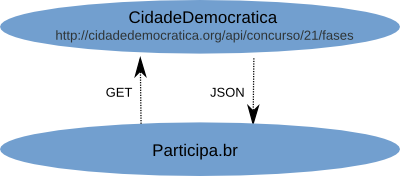
\includegraphics[scale=0.5]{diagrama.png}
\caption{Requisicao a API do Cidade Democrática}
\label{diagrama}
\end{figure}

A partir deste endereço todos os métodos da API estarão acessíveis, a Figura
\ref{diagrama} exemplifica uma requisicao à API a partir do Participa.br,
exemplos de requisição aos métodos da API:

\begin{itemize}
  \item http://cidadedemocratica.org.br/api/concursos
  \item http://cidadedemocratica.org.br/api/concurso/12
  \item http://cidadedemocratica.org.br/api/concurso/12/fases
  \item http://cidadedemocratica.org.br/api/concurso/12/fase/1
\end{itemize}

\subsection{Agregação de dados no Participa.br}

O Participa.br será extendido com uma funcionalidade para leitura dos dados
fornecidos pela API do Cidade Democrática, esta funcionalidade será
desenvolvida como forma de um serviço que ficará lendo periodicamente de forma
automatizada os dados do Cidade Democrática, este serviço irá ser executado
junto ao serviço Noosfero e irá ler a cada 15 minutos os dados do Cidade
Democrática, ou seja irá acessar a API do Cidade Democrática puxando todos os
dados novos desde a última leitura, a identificação de quais são novos será
feito a partir de um controle feito no lado do Noosfero, cada conteúdo
devidamente agregado ao Participa.br será registrado numa tabela do banco de
dados contendo a URI daquele item, a URI dos itens vindos do Cidade
Democrática são únicos, 2 items nunca terão a mesma URI, então este será o
ponto de controle.

O processo será primeiro identificar os concursos existentes no Cidade
Democrática, percorrer cada concurso copiando seus dados, como:

\begin{itemize}
  \item Titulo
  \item Resumo
  \item Conteúdo (como funciona)
  \item Quem propoe
  \item Numero de propostas
  \item Numero de participantes
  \item Tags
  \item Cidade
  \item Estado
\end{itemize}

Além dos dados do próprio concurso, citados acima, serão copiados também os
dados das etapas, que são compostas de:

\begin{itemize}
  \item Data de inicio e fim
  \item Nome da etapa
  \item Contribuições dos participantes (a depender da etapa pode ser: inspiracoes, propostas, comentarios, etc)
\end{itemize}

Cada Concurso possui exatamente 5 etapas, são elas:

\begin{itemize}
  \item Inspiração: os usuários são convidados a enviar imagens para inspirar os participantes do concurso.
  \item Propostas: momento em que as propostas e problemas são enviados para responder ao tema do Concurso e quando também é possível comentar propostas de outros para ajudar a melhorar.
  \item Aplausos: os participantes podem escolher as melhores ideias e dar o seu apoio para quantas quiser.
  \item União: para ganhar força e visibilidade, as ideias que forem semelhantes podem ser unidas em uma só, somando também seus comentários e apoios.
  \item Ganhadores: é quando ficamos sabendo quais foram as ideias e os ganhadores em cada categoria de premiação.
\end{itemize}

Cada contribuição dos participantes em cada fase tem seu próprio conteúdo e
serão também copiados para o Participa.br:

\begin{itemize}
  \item Titulo
  \item Conteudo
  \item Tags
  \item Autor
  \item Fotos
\end{itemize}

Outros usuarios podem apoiar ou comentar cada proposta, estes comentarios
serao tambem copiados para o participa e possui os seguintes dados:

\begin{itemize}
  \item Titulo
  \item Conteudo
  \item Data do comentário
  \item Autor
  \item Tags
\end{itemize}

Este serviço a ser implementado no Participa.br deverá funcionar como {\it
daemon} (ou seja, um serviço executando em background) e irá ler dados via API
do Cidade Democrática a cada 15 minutos, segue abaixo um exemplo de código em
Ruby de como este {\it daemon} deve ser implementado.

\begin{framed}
\begin{lstlisting}[caption=Exemplo de código Ruby para o daemon]
  #!/usr/bin/env ruby
  require 'daemons'
  options = {
    :dir_mode   => :normal,
    :multiple   => false,
    :backtrace  => true,
    :log_output => true,
    :monitor    => false
  }
  Daemons.run_proc(options[:app_name], options) do
    require './config/environment'
    CidadeDemocraticaAPI.new.start
  end
\end{lstlisting}
\end{framed}

Os dados coletados pelo {\it daemon} serão armazenados em uma tabela no banco
de dados do Participa.br, esta tabela deve se chamar {\it concursos} e deve
ter uma estrutura como descrita na Tabela \ref{dados}.

\begin{table}[t]
\centering
\begin{tabular}{|l|l|}
  \hline
  Campo                   & Tipo de dado \\
  \hline
  id                      & inteiro \\
  id original             & inteiro \\
  titulo                  & texto \\
  resumo                  & texto \\
  conteúdo                & texto \\
  quem propoe             & referencia para tabela de pessoas \\
  numero de propostas     & inteiro \\
  numero de participantes & inteiro \\
  tags                    & texto \\
  cidade                  & texto \\
  estado                  & texto \\
  \hline
\end{tabular}
\caption{Especificacao dos campos e tipos de dados para a tabela de concursos}
\label{dados}
\end{table}

O administrador do ambiente poderá configurar o {\it daemon} para copiar e
publicar automaticamente os dados ou pode ativar um mecanismo de moderação,
onde todo conteúdo será copiado para sua tabela correspondente no
banco de dados com uma {\it flag} que indique aguardando moderação, todo conteúdo
aguardando moderação sera gerenciado através de uma interface simples e
intuitiva, como descrito na Figura \ref{moderacao}, esta interface estará
disponível apenas para os administradores do ambiente.

\begin{figure}[h!]
\center
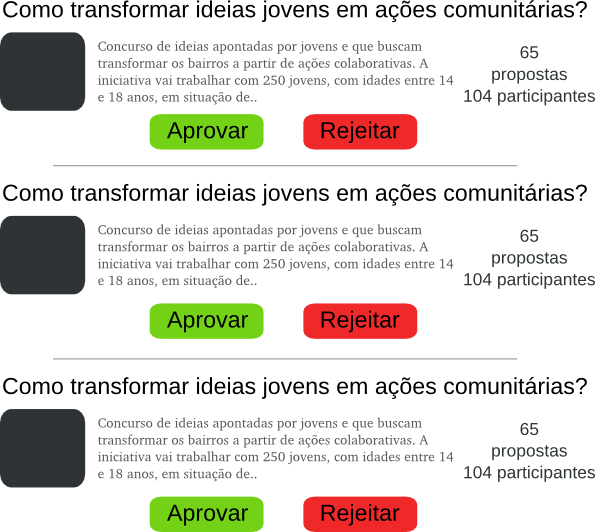
\includegraphics[scale=0.6]{moderacao.png}
\caption{Moderacao de conteúdos no Participa.br}
\label{moderacao}
\end{figure}

Por fim, e não menos importante, é necessário citar a importância semantica de
alguns dos dados a serem copiados pelos mecanismos descritos acima, alguns
destes dados darão uma dimensão temática e federativa ao processo de
agregação, as próximas 2 sessões detalham um pouco sobre isto.

\subsubsection{Dimensão temática}

O Participa.br possui uma forte dimensão social proporcionada pela organização
da plataforma em torno de comunidades e pessoas, o portal é baseado numa
ferramenta de redes sociais e todo o conteúdo é organizado em torno das
comunidades. De tal forma que o contato das pessoas ao portal ocorre a partir
de temas de interesse, onde participam e contribuem com as diversas
comunidades existentes, esta dimensão social é parte essencial da plataforma e
tem sido construída desde a concepção inicial da ferramenta. Apesar disso, a
plataforma ainda carece de uma melhor estrutura para promover uma nova
dimensão, chamada aqui de dimensão temática.  Esta dimensão será construída
através da agregação das {\it tags} vindas do portal Cidade Democrática ao
Participa.br, estas tags serão copiadas para cada conteúdo agregado ao
Participa.br, isso permitirá navegação por temas e dará opções de filtrar
conteúdos por diversos critérios. Esta dimensão temática auxiliará também no
processo de moderação assistida, permitindo o administrador filtar itens
que estão aguardando moderação.

\subsubsection{Dimensão federativa}

\begin{figure}[h!]
\center
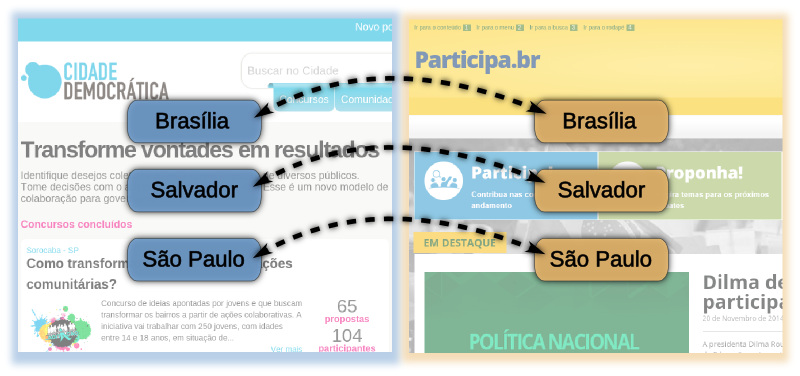
\includegraphics[scale=0.4]{mapeamento-cidades.png}
\caption{Mapeamento de estados, cidades e bairros entre Participa.br e Cidade
Democrática}
\label{mapeamento}
\end{figure}

O Cidade Democrática possui informações sobre estado, cidade e bairro
relacionados a cada tópico, estas informações serão agregadas ao Participa.br
a partir de um mapeamento previamente estabelecido entre cada estado, cidade e
bairro do Cidade Democrática para dados similares no Participa.br. O Noosfero,
plataforma por trás do Participa.br, possui uma entidade chamada {\it Region},
esta entidade é armazenada na tabela {\it categories} do banco de dados e
permite armazenar diversos níveis e sub-níveis de informação, permitindo
simular e replicar a estrutura existende no Cidade Democrática, uma ilustração
sobre este mapeamento é apresentada na Figura \ref{mapeamento}. Este
mapeamento permitirá manter os dados vindos do Cidade Democrática
categorizados por estado, cidade e bairro, dando uma dimensao federativa aos
dados agregados.

\section{Conclusão}

Neste documento foi apresentado um \ProductDescription

Na prática a agregação de dados ao Participa.br vindos do Cidade Democrática
proporcionará aos usuários a capacidade de participar de concultas públicas
realizadas no portal Cidade Democrática através da interface do próprio
Participa.br. De outra forma os usuários seriam obrigados a se cadastrar no
Cidade Democrática para participar e contribuir com tais consultas. Isto iria
levar tais usuários a ter contato com uma interface diferente daquela que já estão
habituados, gerando maior desconforto e dificuldade de participação nos
processos participativos realizados no portal.

Esta agregação irá também potencializar o impacto das consultas realizadas no
Cidade Democrática, oferecendo mais um canal de participação em uma plataforma
com uma ampla base de usuários. Além de proporcionar aos usuários do
Participa.br uma maior oferta de processos participativos, garantindo um maior
volume de mecanismos participativos aos usuários do Participa.br.

Lembramos que para tornar o Portal de Consulta Pública realmente um canal de
consulta e participação popular na discussão e na definição da agenda
prioritária do país, é necessário que além de documentação faça-se um esforço
de movimentar as pessoar fora do ambiente virtual, para que haja um
engajamento no uso e contribuição deste projeto de forma consistente e perene.

\newpage
\bibliography{bibliografia}
\newpage
\listoffigures
\newpage
\printindex

\end{document}
